\documentclass[11pt]{article}

\usepackage{amsmath,amssymb}
\usepackage{mathtools}
\usepackage[dvipdfmx]{graphicx}

\title{Boundary Condition for Entry Interface}
\author{Ryo Nakamura}
\date{October 16, 2019}

\begin{document}
\maketitle
\section{(Geo)Detic Latitude / Altitude \cite{dalt}\cite{dlat}}
Given a probe position in fixed coordinate as $(x, y, z)$, the (geo)centric latitude is written as
\begin{equation}
	\label{eq:geo_lat}
	\begin{aligned}
		\phi_c = \arctan{\frac{y}{x}}
	\end{aligned}
\end{equation}
Using the equatorial radius $R$ and flattening $f$, $x_a$ in Figure \ref{fig:1} is written as
\begin{equation}
	\label{eq:x_a}
	\begin{aligned}
		x_a = \frac{(1-f)R}{\sqrt{\tan^{2}{\phi_c}+(1-f)^2}}
	\end{aligned}
\end{equation}
Using the relationship between (geo)centric latitude at the planet's surface and (geo)detic latitude, $\phi_{dg}$ is written as
\begin{equation}
	\label{eq:phi_dg}
	\begin{aligned}
		\phi_{dg} =\arctan{\left(\frac{\tan{\phi_c}}{(1-f)^2}\right)}
	\end{aligned}
\end{equation}
The radius $r_a$ from the center of the planet (O) to the surface of the planet (S) in Figure \ref{fig:1} is calculated by using trigonometric relationship.
\begin{equation}
	\label{eq:r_a}
	\begin{aligned}
		r_a = \frac{x_a}{\cos{\phi_c}}
	\end{aligned}
\end{equation}
The distance from (S) to (P) in Figure \ref{fig:1} is defined by
\begin{equation}
	\label{eq:l}
	\begin{aligned}
		l = r - r_a
	\end{aligned}
\end{equation}
The angular difference between (geo)centric latitude and (geo)detic latitude at (S) in Figure \ref{fig:1} is defined by
\begin{equation}
	\label{eq:delta_phi_g}
	\begin{aligned}
	\delta\phi_g = \phi_{dg} - \phi_c
	\end{aligned}
\end{equation}
The equation for the radius of curvature in the Meridian at $\phi_{dg}$ (distance between (S) and (W) in Figure \ref{fig:1}) is written as
\begin{equation}
	\label{eq:rho_a}
	\begin{aligned}
	\rho_a = \frac{R(1-f)^2}{\left(1-(2f-f^2)\sin^2{\phi_{dg}}\right)^{3/2}}
	\end{aligned}
\end{equation}

\noindent Then the (geo)detic latitude is calculated with
\begin{equation}
	\label{eq:phi_d}
	\begin{aligned}
	\phi_d = \phi_{dg} - \delta\phi
	\end{aligned}
\end{equation}
,where
\begin{equation}
	\label{eq:delta_phi}
	\begin{aligned}
	\delta\phi = \arctan{\left(\frac{l\sin{\delta\phi_g}}{\rho_a+l\cos{\delta\phi_g}}\right)}
	\end{aligned}
\end{equation}

\noindent The (geo)detic altitude above the planetary ellipsoid is calculated with
\begin{equation}
	\label{eq:geo_alt}
	\begin{aligned}
	h =\sqrt{x^2+y^2}\cos{\phi_d} + \left(z + (2f-f^2)N\sin{\phi_d}\right)\sin{\phi_d} - N
	\end{aligned}
\end{equation}
,where the radius of curvature in the vertical prime $N$ (distance between (T) and (V) in Figure \ref{fig:1}) is written as
\begin{equation}
	\label{eq:N}
	\begin{aligned}
	N =\frac{R}{\sqrt{1-(2f-f^2)\sin^2{\phi_d}}}
	\end{aligned}
\end{equation}

\begin{figure}
  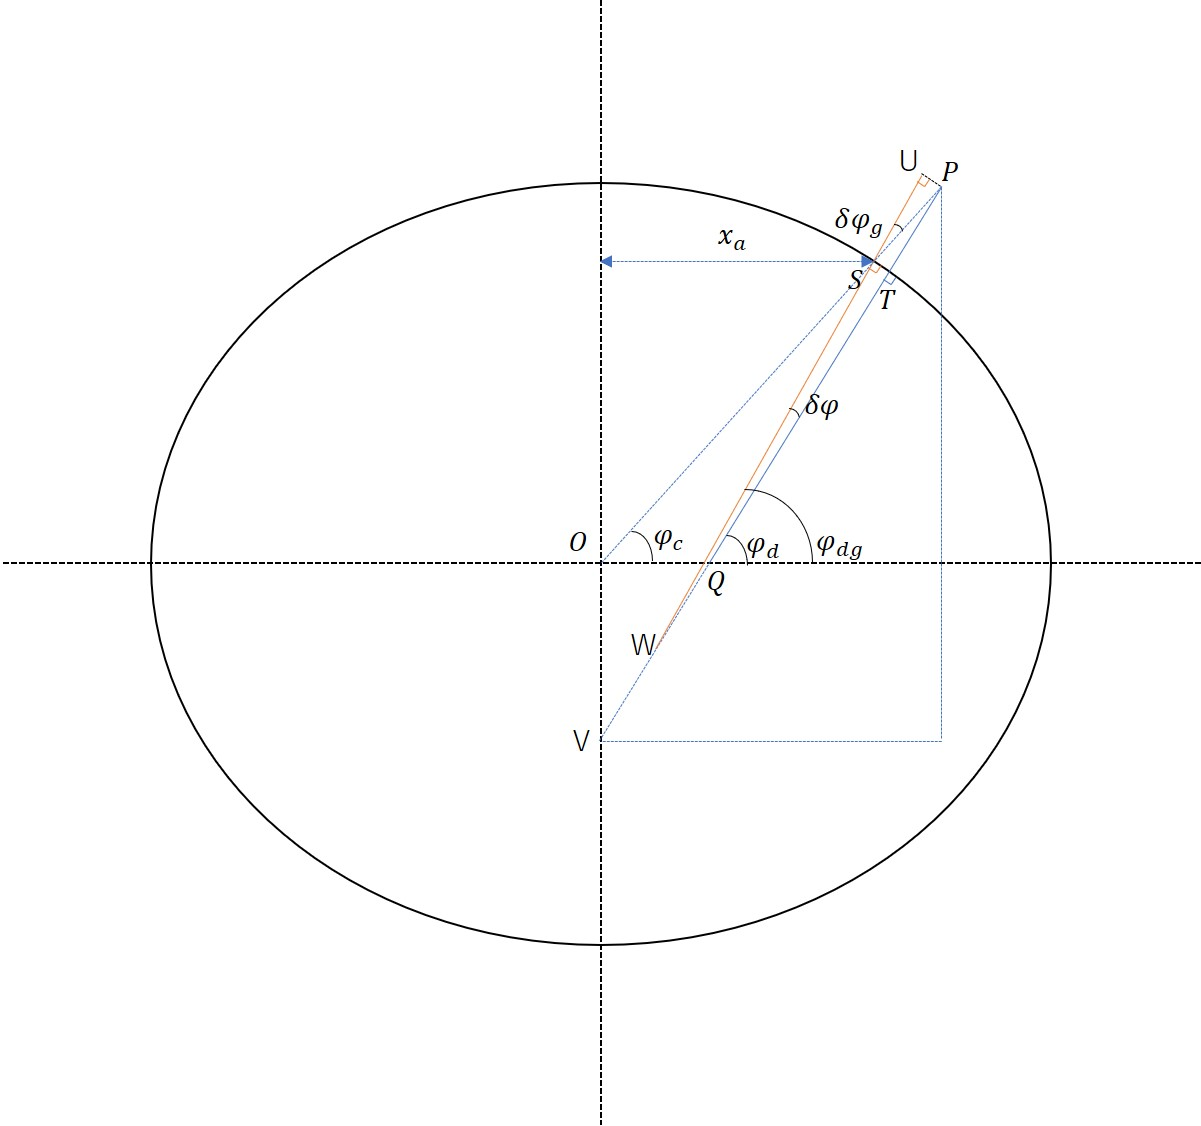
\includegraphics[width=\linewidth]{fig1.jpg}
  \caption{Geometry of (geo)detic latitude and altitude}
  \label{fig:1}
\end{figure}

\section{Velocity vector}
\subsection{Magnitude}
The magnitude of the entry inertial velocity vector and its derivatives are written as
\begin{equation}
	\label{eq:velocity_magnitude}
	\begin{aligned}
		&v = \left|\vec{v}\right| = \sqrt{v_{x}^{2}+v_{y}^{2}+v_{z}^{2}}\\
		&\frac{\partial{v_r}}{\partial{\vec{v}}} = \frac{\vec{v_{r}}}{v_r}
	\end{aligned}
\end{equation}


\subsection{Azimuth in spherical local coordinate}\label{Azimuth}
The azimuth angle $Az$ of the inertial velocity vector in spherical coordinate is written as
\begin{equation}
	\label{eq:velocity_Az}
	\begin{aligned}
		&Az = \arctan{\frac{v_{east}}{v_{north}}}
	\end{aligned}
\end{equation}
,where $v_{east}$ and $v_{north}$ are inertial velocity elements at the spherical local coordinate as
\begin{equation}
	\label{eq:velocity_local}
	\begin{aligned}
		\begin{bmatrix}
		v_{up}\\
		v_{east}\\
		v_{north}
		\end{bmatrix} =
		\begin{bmatrix}
		\cos{\phi} & 0 & \sin{\phi}\\
		0 & 1 & 0\\
		-\sin{\phi} & 0 & \cos{\phi}
		\end{bmatrix}
		\begin{bmatrix}
		\cos{\lambda} & \sin{\lambda} & 0\\
		-\sin{\lambda}& \cos{\lambda} & 0\\
		0 & 0 & 1
		\end{bmatrix}
		\begin{bmatrix}
		v_{r}\\
		v_{r}\\
		v_{r}
		\end{bmatrix}
	\end{aligned}
\end{equation}
Here, $\phi$ is a (geo)centric latitude and $\lambda$ is a longitude.

\noindent The derivative of azimuth angle is written as
\begin{equation}
	\label{eq:velocity_Az_deriv}
	\begin{aligned}
		\frac{\partial Az}{\partial *} = \frac{v_{north}^2}{v_{north}^2 + v_{east}^2}
		\left(
		\frac{1}{v_{north}} \frac{\partial v_{east}}{\partial *} - \frac{v_{east}}{v_{north}^2} \frac{\partial v_{north}}{\partial *}
		\right)
	\end{aligned}
\end{equation}
,where derivatives of these local velocity elements are written as
\begin{equation}
	\label{eq:velocity_local_deriv}
	\begin{aligned}
	\frac{\partial}{\partial *}
		\begin{bmatrix}
		v_{up}\\
		v_{east}\\
		v_{north}
		\end{bmatrix} =
		\begin{bmatrix}
		-\sin{\phi}\frac{\partial \phi}{\partial *} & 0 & \cos{\phi}\frac{\partial \phi}{\partial *}\\
		0 & 0 & 0\\
		-\cos{\phi}\frac{\partial \phi}{\partial *} & 0 & -\sin{\phi}\frac{\partial \phi}{\partial *}
		\end{bmatrix}
		\begin{bmatrix}
		\cos{\lambda} & \sin{\lambda} & 0\\
		-\sin{\lambda}& \cos{\lambda} & 0\\
		0 & 0 & 1
		\end{bmatrix}
		\begin{bmatrix}
		v_{x}\\
		v_{y}\\
		v_{z}
		\end{bmatrix} \\
		+
		\begin{bmatrix}
		\cos{\phi} & 0 & \sin{\phi}\\
		0 & 1 & 0\\
		-\sin{\phi} & 0 & \cos{\phi}
		\end{bmatrix}
		\begin{bmatrix}
		-\sin{\lambda}\frac{\partial \lambda}{\partial *} & \cos{\lambda}\frac{\partial \phi}{\partial *} & 0\\
		-\cos{\lambda}\frac{\partial \phi}{\partial *}& -\sin{\lambda}\frac{\partial \phi}{\partial *} & 0\\
		0 & 0 & 0
		\end{bmatrix}
		\begin{bmatrix}
		v_{x}\\
		v_{y}\\
		v_{z}
		\end{bmatrix}
	\end{aligned}
\end{equation}
\begin{equation}
	\begin{aligned}
	\frac{\partial}{\partial \vec{v}}
		\begin{bmatrix}
		v_{up}\\
		v_{east}\\
		v_{north}
		\end{bmatrix} =
		\begin{bmatrix}
		\cos{\phi} & 0 & \sin{\phi}\\
		0 & 1 & 0\\
		-\sin{\phi} & 0 & \cos{\phi}
		\end{bmatrix}
		\begin{bmatrix}
		\cos{\lambda} & \sin{\lambda} & 0\\
		-\sin{\lambda}& \cos{\lambda} & 0\\
		0 & 0 & 1
		\end{bmatrix}
	\end{aligned}
\end{equation}

\subsection{Horizontal Flight Path Angle in spherical local coordinate}
The horizontal flight path angle $HFPA$ of the inertial velocity vector in spherical coordinate is written as
\begin{equation}
	\label{eq:velocity_HFPA}
	\begin{aligned}
		HFPA &= \arctan{\frac{v_{up}}{\sqrt{v_{north}^2 + v_{east}^2}}}\\
		&=\arccos{\frac{\vec{r}\cdot\vec{v}}{|\vec{r}||\vec{v}|}}
	\end{aligned}
\end{equation}

\noindent The derivative of horizontal flight path angle is written as

\begin{equation}
	\label{eq:velocity_HFPA_deriv}
	\begin{aligned}
		\frac{\partial HFPA}{\partial *} =
		\frac{\sqrt{v_{north}^2 + v_{east}^2}}{v_{north}^2 + v_{east}^2 + v_{up}^2}
		\left(
		\frac{\partial v_{up}}{\partial *}
		- \frac{v_{up}}{v_{north}^2 + v_{east}^2}
		\left(
		v_{north}\frac{\partial v_{north}}{\partial *} + v_{east}\frac{\partial v_{east}}{\partial *}
		\right)
		\right)
	\end{aligned}
\end{equation}
The derivatives of the local velocity elements are same with those in \ref{Azimuth}

\subsection{Vertical Flight Path Angle in spherical local coordinate}
The vertical flight path angle $VFPA$ of the inertial velocity vector in spherical coordinate is written as
\begin{equation}
	\label{eq:velocity_VFPA}
	\begin{aligned}
		VFPA &=\arccos{\frac{\vec{r}\cdot\vec{v}}{|\vec{r}||\vec{v}|}}
	\end{aligned}
\end{equation}

\noindent The derivative of $\cos{\left(VFPA\right)}$ is written as

\begin{equation}
	\label{eq:velocity_VFPA_deriv}
	\begin{aligned}
		\frac{\partial \cos{\left(VFPA\right)}}{\partial \vec{r}} &=
		\frac{\vec{v}}{|\vec{r}||\vec{v}|} - \frac{\vec{r}\cdot\vec{v}}{|\vec{r}|^2|\vec{v}|}
		\frac{\partial |\vec{r}|}{\partial \vec{r}}\\
		\frac{\partial \cos{\left(VFPA\right)}}{\partial \vec{v}} &=
		\frac{\vec{r}}{|\vec{r}||\vec{v}|} - \frac{\vec{r}\cdot\vec{v}}{|\vec{r}||\vec{v}|^2}
		\frac{\partial |\vec{v}|}{\partial \vec{v}}
	\end{aligned}
\end{equation}

\section{Relative velocity vector}
The entry velocity vector of a vehicle relative to the Earth ground (or atmosphere) is written as
\begin{equation}
	\label{eq:rel_velocity}
	\begin{aligned}
		\vec{v_r} = \vec{v} - \vec{\omega} \times \vec{r} = \vec{v} -
		\begin{bmatrix}
		0 & -\omega_3 & \omega_2 \\
		\omega_3 & 0 & -\omega_1 \\
		-\omega_2 & \omega_1 & 0
		\end{bmatrix}
		\vec{r}
	\end{aligned}
\end{equation}
\subsection{Magnitude}
The magnitude of the relative velocity vector and its derivatives are written as
\begin{equation}
	\label{eq:rel_velocity_magnitude}
	\begin{aligned}
		&v_r = \left|\vec{v_r}\right| = \sqrt{v_{rx}^{2}+v_{ry}^{2}+v_{rz}^{2}}\\
		&\frac{\partial{v_r}}{\partial{\vec{r}}} =
		\begin{bmatrix}
		0 & -\omega_3 & \omega_2 \\
		\omega_3 & 0 & -\omega_1 \\
		-\omega_2 & \omega_1 & 0
		\end{bmatrix}
		\frac{\partial{v_r}}{\partial{\vec{v_r}}}\\
		&\frac{\partial{v_r}}{\partial{\vec{v}}} = \frac{\vec{v_{r}}}{v_r}
	\end{aligned}
\end{equation}


\subsection{Azimuth in (geo)detic local coordinate}\label{Detic Azimuth}
The azimuth angle of the relative velocity vector $Az$ is written as
\begin{equation}
	\label{eq:rel_velocity_Az}
	\begin{aligned}
		&Az = \arctan{\frac{v_{r_{east}}}{v_{r_{north}}}}
	\end{aligned}
\end{equation}
,where $v_{r_{east}}$ and $v_{r_{north}}$ are relative velocity elements at the horizontal local coordinate as
\begin{equation}
	\label{eq:rel_velocity_local}
	\begin{aligned}
		\begin{bmatrix}
		v_{r_{up}}\\
		v_{r_{east}}\\
		v_{r_{north}}
		\end{bmatrix} =
		\begin{bmatrix}
		\cos{\phi} & 0 & \sin{\phi}\\
		0 & 1 & 0\\
		-\sin{\phi} & 0 & \cos{\phi}
		\end{bmatrix}
		\begin{bmatrix}
		\cos{\lambda} & \sin{\lambda} & 0\\
		-\sin{\lambda}& \cos{\lambda} & 0\\
		0 & 0 & 1
		\end{bmatrix}
		\begin{bmatrix}
		v_{rx}\\
		v_{ry}\\
		v_{rz}
		\end{bmatrix}
	\end{aligned}
\end{equation}
Here, $\phi$ is a (geo)detic latitude and $\lambda$ is a longitude.

\noindent The derivative of azimuth angle is written as
\begin{equation}
	\label{eq:rel_velocity_Az_deriv}
	\begin{aligned}
		\frac{\partial Az}{\partial *} = \frac{v_{r_{north}}^2}{v_{r_{north}}^2 + v_{r_{east}}^2}
		\left(
		\frac{1}{v_{r_{north}}} \frac{\partial v_{r_{east}}}{\partial *} - \frac{v_{r_{east}}}{v_{r_{north}}^2} \frac{\partial v_{r_{north}}}{\partial *}
		\right)
	\end{aligned}
\end{equation}
,where derivatives of these local velocity elements are written as
\begin{equation}
	\label{eq:rel_velocity_local_deriv}
	\begin{aligned}
	\frac{\partial}{\partial *}
		\begin{bmatrix}
		v_{r_{up}}\\
		v_{r_{east}}\\
		v_{r_{north}}
		\end{bmatrix} =
		\begin{bmatrix}
		-\sin{\phi}\frac{\partial \phi}{\partial *} & 0 & \cos{\phi}\frac{\partial \phi}{\partial *}\\
		0 & 0 & 0\\
		-\cos{\phi}\frac{\partial \phi}{\partial *} & 0 & -\sin{\phi}\frac{\partial \phi}{\partial *}
		\end{bmatrix}
		\begin{bmatrix}
		\cos{\lambda} & \sin{\lambda} & 0\\
		-\sin{\lambda}& \cos{\lambda} & 0\\
		0 & 0 & 1
		\end{bmatrix}
		\begin{bmatrix}
		v_{rx}\\
		v_{ry}\\
		v_{rz}
		\end{bmatrix} \\
		+
		\begin{bmatrix}
		\cos{\phi} & 0 & \sin{\phi}\\
		0 & 1 & 0\\
		-\sin{\phi} & 0 & \cos{\phi}
		\end{bmatrix}
		\begin{bmatrix}
		-\sin{\lambda}\frac{\partial \lambda}{\partial *} & \cos{\lambda}\frac{\partial \phi}{\partial *} & 0\\
		-\cos{\lambda}\frac{\partial \phi}{\partial *}& -\sin{\lambda}\frac{\partial \phi}{\partial *} & 0\\
		0 & 0 & 0
		\end{bmatrix}
		\begin{bmatrix}
		v_{rx}\\
		v_{ry}\\
		v_{rz}
		\end{bmatrix} \\
		+
		\begin{bmatrix}
		\cos{\phi} & 0 & \sin{\phi}\\
		0 & 1 & 0\\
		-\sin{\phi} & 0 & \cos{\phi}
		\end{bmatrix}
		\begin{bmatrix}
		\cos{\lambda} & \sin{\lambda} & 0\\
		-\sin{\lambda}& \cos{\lambda} & 0\\
		0 & 0 & 1
		\end{bmatrix}
		\begin{bmatrix}
		\frac{\partial v_{rx}}{\partial *}\\
		\frac{\partial v_{ry}}{\partial *}\\
		\frac{\partial v_{rz}}{\partial *}
		\end{bmatrix}
	\end{aligned}
\end{equation}
\begin{equation}
	\begin{aligned}
	\frac{\partial}{\partial \vec{v}}
		\begin{bmatrix}
		v_{r_{up}}\\
		v_{r_{east}}\\
		v_{r_{north}}
		\end{bmatrix} =
		\begin{bmatrix}
		\cos{\phi} & 0 & \sin{\phi}\\
		0 & 1 & 0\\
		-\sin{\phi} & 0 & \cos{\phi}
		\end{bmatrix}
		\begin{bmatrix}
		\cos{\lambda} & \sin{\lambda} & 0\\
		-\sin{\lambda}& \cos{\lambda} & 0\\
		0 & 0 & 1
		\end{bmatrix}
	\end{aligned}
\end{equation}

\subsection{Horizontal Flight Path Angle in (geo)detic local coordinate}
The horizontal flight path angle of the relative velocity vector $HFPA$ is written as
\begin{equation}
	\label{eq:rel_velocity_HFPA}
	\begin{aligned}
		&HFPA = \arctan{\frac{v_{r_{up}}}{\sqrt{v_{r_{north}}^2 + v_{r_{east}}^2}}}
	\end{aligned}
\end{equation}

\noindent The derivative of horizontal flight path angle is written as

\begin{equation}
	\label{eq:rel_velocity_HFPA_deriv}
	\begin{aligned}
		\frac{\partial HFPA}{\partial *} =
		\frac{\sqrt{v_{r_{north}}^2 + v_{r_{east}}^2}}{v_{r_{north}}^2 + v_{r_{east}}^2 + v_{r_{up}}^2}
		\left(
		\frac{\partial v_{r_{up}}}{\partial *}
		- \frac{v_{r_{up}}}{v_{r_{north}}^2 + v_{r_{east}}^2}
		\left(
		v_{r_{north}}\frac{\partial v_{r_{north}}}{\partial *} + v_{r_{east}}\frac{\partial v_{r_{east}}}{\partial *}
		\right)
		\right)
	\end{aligned}
\end{equation}
The derivatives of the local velocity elements are same with those in \ref{Detic Azimuth}

\begin{thebibliography}{99}
	\bibitem{dalt} https://jp.mathworks.com/help/aeroblks/ecefpositiontolla.html
  \bibitem{dlat} https://jp.mathworks.com/help/aeroblks/geocentrictogeodeticlatitude.html
\end{thebibliography}

\end{document}
